  \algrenewcommand\algorithmicindent{0.5em}%
  \algnewcommand\algorithmicforeach{\textbf{for each}}
\algdef{S}[FOR]{ForEach}[1]{\algorithmicforeach\ #1\ \algorithmicdo}
\begin{figure}[t]%[b]
% \begin{algorithm}[H]
% \algsetup{linenosize=\tiny}
  % \scriptsize
  % \newcommand{\pluseq}{\mathrel{+}=}
\center
\footnotesize
% \hspace{-0.23cm}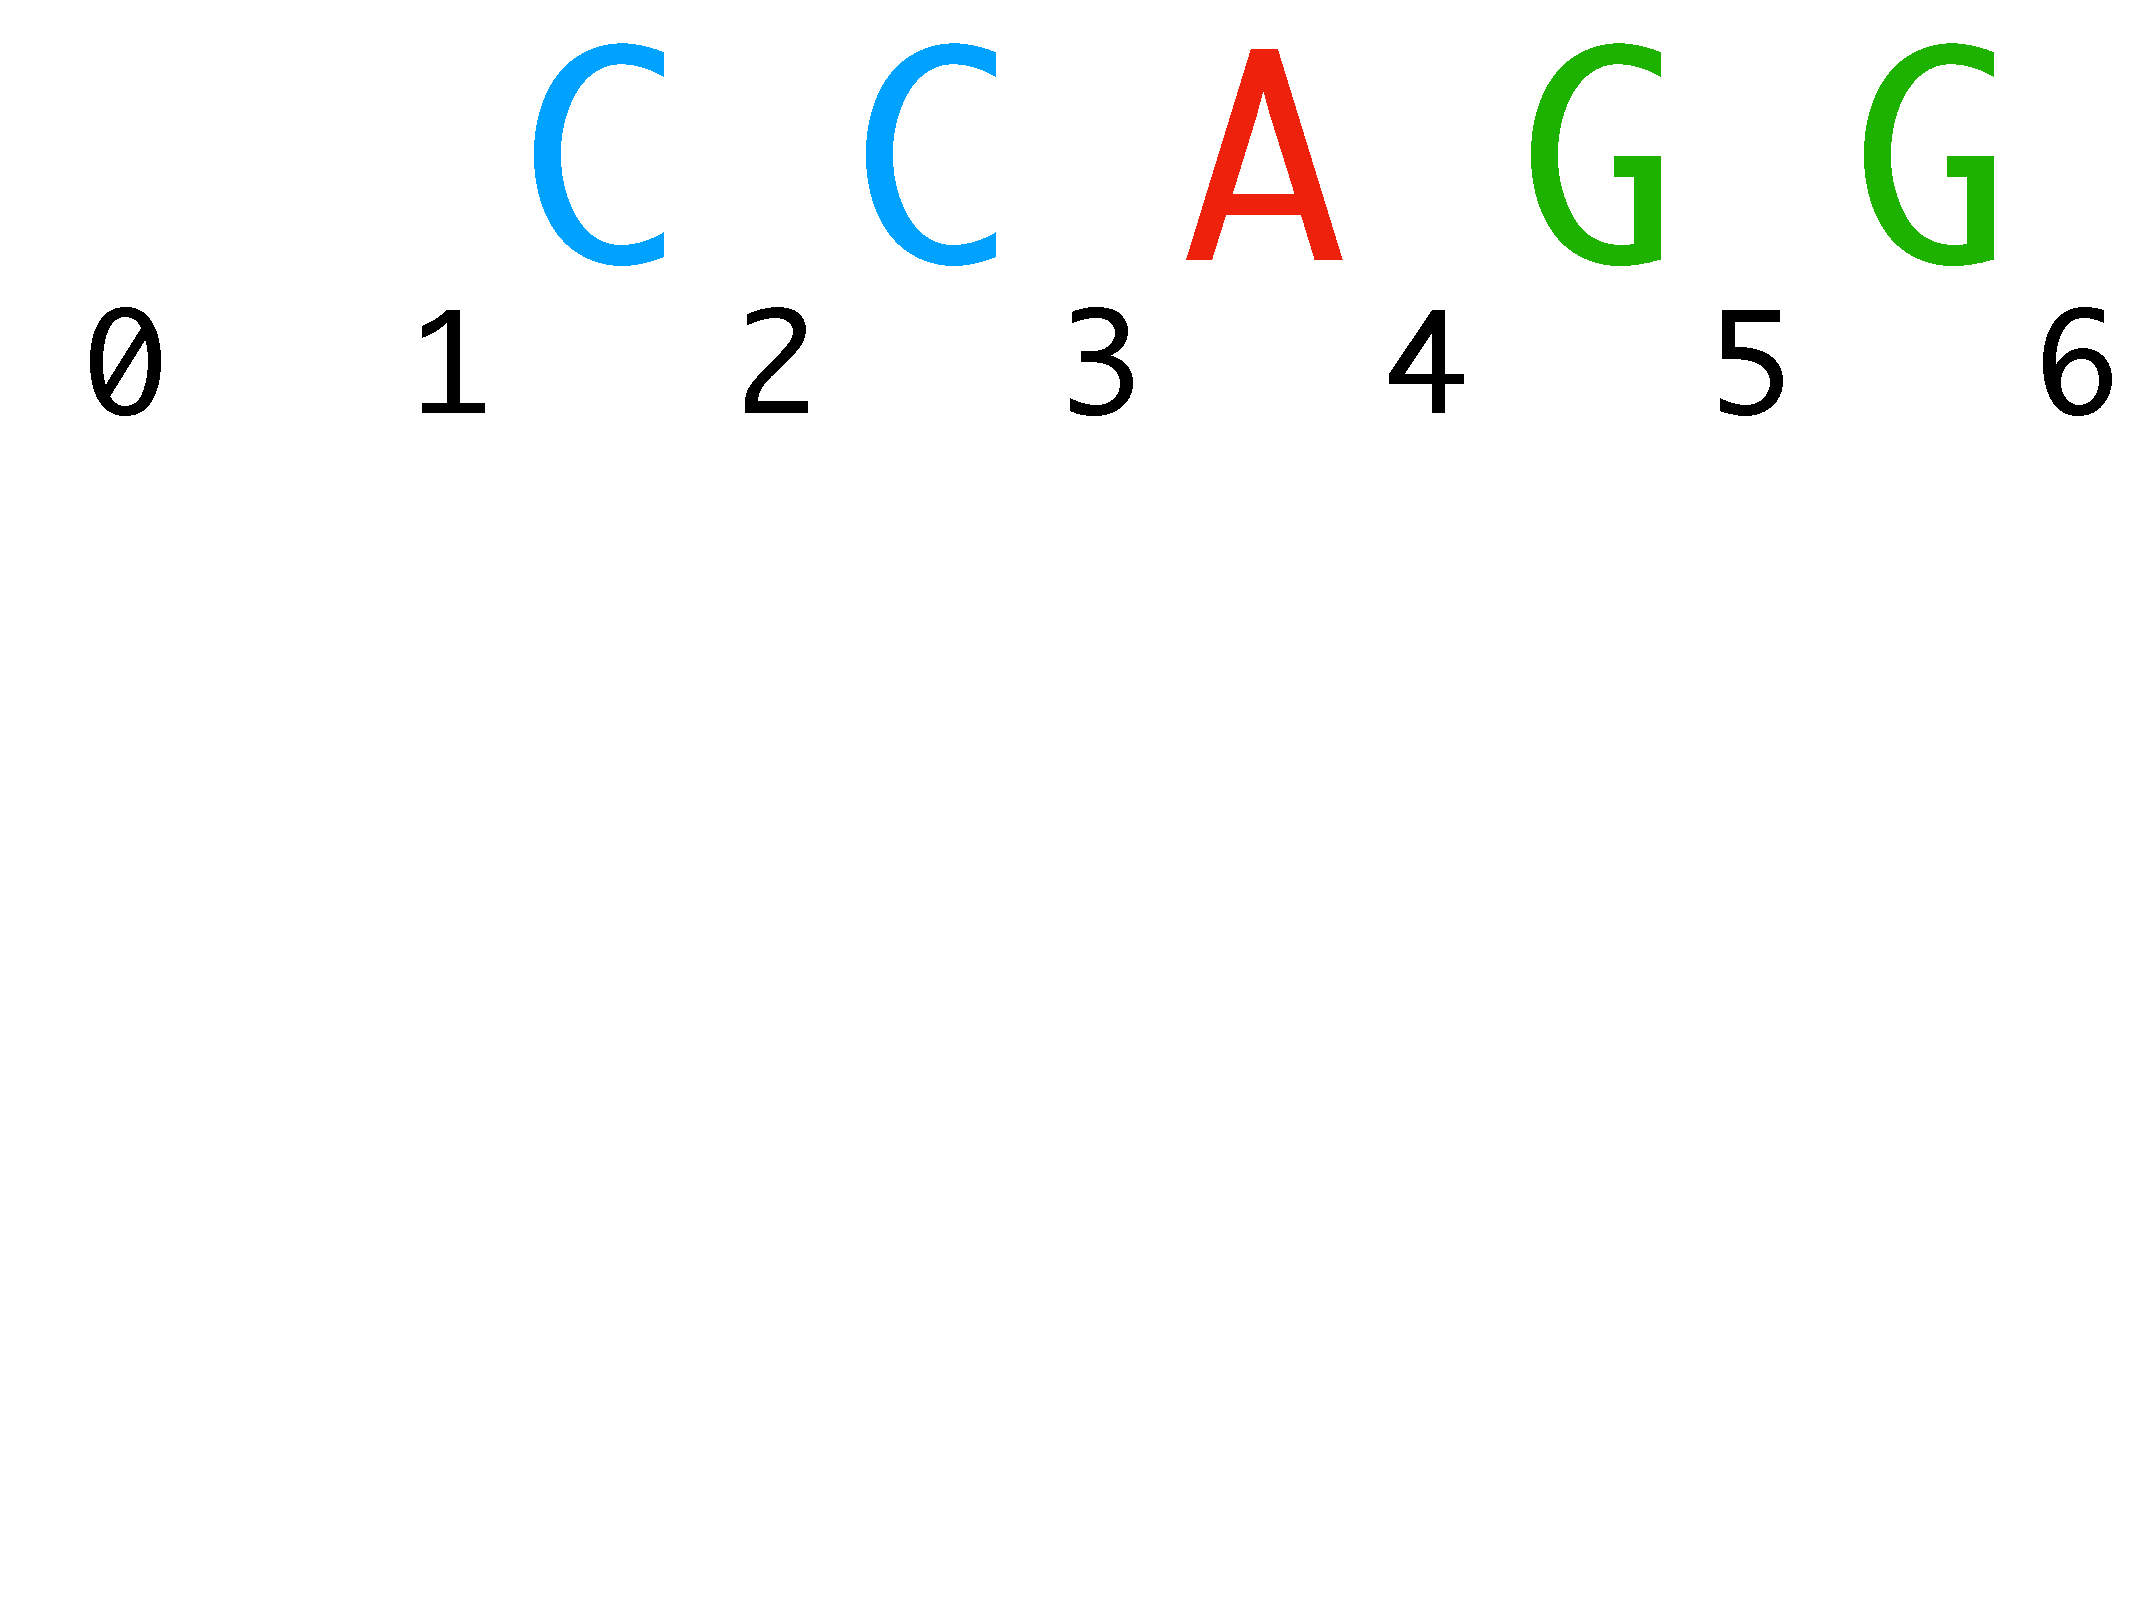
\includegraphics[scale=.16]{figs/index} \\[-3.cm]
%\hspace{-0.23cm}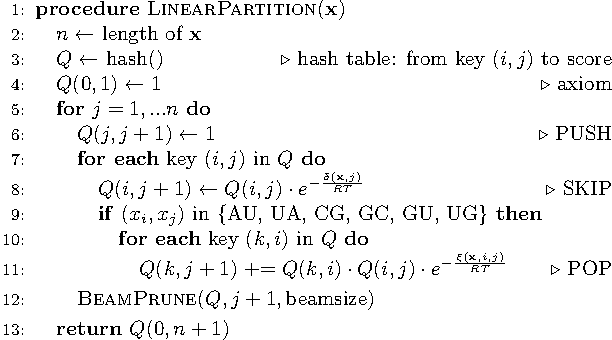
\includegraphics[scale=.83]{figs/algorithm} \\[0.2cm]
\begin{algorithmic}[1]
  \newcommand{\INDSTATE}[1][1]{\State\hspace{#1\algorithmicindent}}
  \setstretch{1.05} % lhuang: usepackage setspace
\Function{LinearPartition}{$\vecx, b$} \Comment{$b$ is the beam size}
% \bindent
    \State $n \gets$ length of $\mathbf x$
    \State $Q \gets$ hash() \Comment{hash table: from span $[i,j]$ to $\Qf{i}{j}$}
    \State $\Qf{j}{j-1} \gets 1$ for all $j$ in $1...n$ \Comment{base cases} \label{line:base}
    \For{$j=1 ... n$}
    \ForEach {$i$ such that $[i,\,j-1]$ in $Q$} \Comment{$O(b)$ iterations}
        \smallskip 
            \State $\Qf{i}{j} \pluseq \Qf{i}{j-1} \cdot e^{-\frac{\delta(\vecx,j)}{RT}} $ \Comment{\nskip} \label{line:skip}
            \If{$x_{i-1}x_j$ in \{AU, UA, CG, GC, GU, UG\}}  \label{line:pair}
                % \State $Q_{i,\,j+1} \gets  C(i,\,j) \cdot e^{-\frac{\xi(\vecx,i,\,j)}{RT}} $
                \ForEach{$k$ such that $[k,\,i-2]$ in $Q$} \Comment{$O(b)$ iters} \smallskip 
                    \State $\Qf{k}{j} \pluseq {\Qf{k}{i-2} \cdot \Qf{i}{j-1} \cdot e^{-\frac{\xi(\vecx,i-1,j)}{RT}}} $ \Comment{\pop} \label{line:pop}
                    % \State $C(0,j+1) \pluseq {C(0,k) \cdot C(k,j+1) \cdot e^{-\frac{\xi(\vecx,i,\,j)}{RT}}} $
                \EndFor
                % \State $C(0,j+1) \pluseq C(0,i) \cdot Q_{i,j+1}$ \Comment{COMBINE}
            \EndIf
        \EndFor
        \State $\textsc {BeamPrune}(Q,j, b)$ \Comment{choose top $b$ out of $Q(\cdot,j)$} \label{line:beamprune}%{see Fig.~\ref{fig:beam_prune_alg}}
        \EndFor
        \vspace{-0.1cm}
    \State \Return $Q$ \Comment{partition function $Q(\vecx)=\Qf{1}{n}$}
% \eindent
\EndFunction
\end{algorithmic}
% \end{algorithm}
\caption{
Partition function calculation pseudocode of a simplified version of the \linearpartition %linear-time partition function calculation
algorithm (the inside phase).
See Fig.~\ref{fig:beam_prune_alg} for the pseudocode of beam pruning (line~\ref{line:beamprune}).
The base-pairing probabilities are computed with the combination of the outside phase
(Fig.~\ref{fig:outside}).
% as well as a beam prune algorithm. 
% Here we model hash tables following Python dictionaries, where $(i, j) \in C$ checks whether the key $(i, j)$ is in the hash $C$; 
% this is needed to ensure linear runtime. 
% Quick select algotithm is used in beam prune, 
% and we skip the details for quick select here since it is well known.
% Real \linearpartition system is much more involved, but the pseudocode illustrates the left-to-right partition function calculation idea using a Nussinov-like fashion.
The actual algorithm using the Turner model is available on \href{https://github.com/LinearFold/LinearPartition}{GitHub}.
%See Fig.~\ref{fig:beam_prune_alg} for {\sc BEAMPRUNE} function.
\label{fig:algorithm}}
\vspace{-.3cm}
% \end{figure*}
\end{figure}
